\RequirePackage[T1]{fontenc}
\documentclass[journal,10pt]{IEEEtran}
\usepackage{mathptmx}
\usepackage{amsmath,amssymb,booktabs,array,multirow}
\usepackage{graphicx,xcolor}
\usepackage{algorithm,algpseudocode}
\usepackage{cite,url}
\usepackage[hidelinks]{hyperref}
\usepackage{tikz}
\usetikzlibrary{arrows.meta,positioning,fit,calc}
\newcommand{\LEAF}{\textsc{LEAF}}
\hyphenation{multi-agent gene-ra-li-za-tion re-pre-sen-ta-tion}
\hypersetup{pdftitle={LEAF: Looped Entity Attention Fusion for Population-Generalizable Multi-Agent Defense},pdfauthor={}}
\begin{document}
\title{LEAF: Looped Entity Attention Fusion for Population-Generalizable Multi-Agent Defense}
\author{Anonymous Authors}
\bstctlcite{leafBibliographyControl}
\maketitle
\markboth{Anonymous Manuscript Submitted for Review}{LEAF: Looped Entity Attention Fusion}
\begin{abstract}
Cooperative target protection requires a policy to coordinate defenders as the numbers of vehicles and protected targets change. We present Looped Entity Attention Fusion (LEAF), an entity-based value-learning method that repeatedly refines receiver-relative entity representations using one shared attention block. A self-conditioned reader accesses the intermediate representations, and learned fusion augments the feature entering a recurrent utility network. Reading depends on the current self representation, while the downstream recurrent state supplies temporal context. Training samples one to four refinement rounds, and standard evaluation uses four. In the HAD simulator, policies trained with at most ten vehicles per team and three targets are evaluated without retraining on 24 configurations, including 50 vehicles per team and 12 targets. Across three training seeds, LEAF improves mean reward over REFIL by 0.800, 1.635, and 2.211 in target, vehicle, and joint extrapolation, respectively. Architectural comparisons and episode-level measurements associate these gains with fewer friendly-collision deaths, more attacker interceptions, and lower first-damage incidence. Frozen interventions reveal reliance on relational features and downstream memory, with most readout weight assigned to the first two rounds.
\end{abstract}
\noindent\textbf{Note to Practitioners---}
Cooperative protection systems may need to reuse a controller when the numbers of defending vehicles, incoming vehicles, and protected assets change. This work provides a shared policy interface that accepts a variable-size set of public entity states. Each defender refines the observed scene, reads it from its own perspective, and updates an individual recurrent state before choosing an action. No explicit population-count encoding or recurrent-state input to the reader is required by the evaluated main method. The controller is trained on small simulated engagements and evaluated with frozen parameters in larger engagements. Reward is the negative of accumulated target damage; friendly-collision deaths are reported separately to expose an operational tradeoff. The evidence concerns a planar simulator, public entity-state observations, and a fixed reactive attacker. Deployment on physical platforms would additionally require sensing and action-interface validation, as well as measured control-cycle timing. The current experiments establish simulated population transfer and describe the associated behavior; they do not establish real-time operation or robustness to an adaptive opponent.
\par
\begin{IEEEkeywords}
Multi-agent reinforcement learning, cooperative control, population generalization, entity attention, target protection.
\end{IEEEkeywords}
\section{Introduction}
\IEEEPARstart{C}{ooperative} target protection requires defenders to redistribute their effort as vehicle and target populations change. An approaching attacker may already be covered by a teammate, while another threatens an exposed asset. Actions therefore depend on relationships among attackers, targets, and defenders, interpreted from the perspective of the defender choosing an action. A policy trained in small engagements must handle different distributions of these relationships when deployed with more vehicles or targets. Reusing one policy across these populations is a concrete requirement for automated cooperative protection.

Entity-based policies provide a common interface to changing scenes. Set encoders and attention accommodate variable entity populations~\cite{zaheer2017deepsets,lee2019settransformer}, and REFIL encourages reuse of interaction patterns through randomized entity-wise value factorization~\cite{iqbal2021refil}. Supporting a larger input set does not itself establish effective coordination. The controller must develop entity context and extract information relevant to the receiving defender. Repeated relational attention offers one way to process that context~\cite{zambaldi2019relational,dehghani2019universal}.

A second question is which processing stages should supply the decision feature. Retaining intermediate representations permits aggregation across depth~\cite{xu2018jk}. Image-classification networks can change correct intermediate predictions into incorrect final predictions~\cite{kaya2019overthinking}; pure-attention rank-loss results also show that depth effects depend on architectural conditions, including residual and feedforward paths~\cite{dong2021attention}. These precedents motivate exposing intermediate contexts without assuming that the last context is always preferable. They do not establish those phenomena in a cooperative policy.

A third requirement concerns time. Public physical states need not reveal an attacker's assigned target, motivating memory across observations. Processing the current entity set and retaining temporal information are different operations. We place the relational reader before the recurrent utility network, allowing its query to depend on the current self representation while the downstream GRU retains history across physical decisions.

\textbf{Looped Entity Attention Fusion (LEAF)} combines these three roles. Each defender initializes a receiver-relative entity workspace, applies a shared contextual-update block, and reads its intermediate sets with one self-conditioned query. Learned weights fuse the reads, and a residual projection augments the REFIL feature before one GRU update. The query's previous-GRU-state input is zero and explicit count injection is disabled; downstream recurrence is retained. Fusion selects information from the computed rounds without changing execution depth. Training samples one through four rounds, and standard evaluation uses four. Figure~\ref{fig:framework} shows this separation of within-decision processing and cross-decision memory.

We evaluate frozen policies in HAD target protection against a fixed reactive attacker. Across three training seeds, LEAF has higher group mean reward $R=-D$, where $D$ is accumulated target damage, than five learning baselines and Rule in ID, target-count, vehicle-count, and joint extrapolation. Evaluation reaches five times the largest training vehicle population and four times the largest training target count, without retraining. Saved-design comparisons examine entity-context updating, query-history placement, and host integration; the complete variant results retain the context in which LEAF was selected.

Frozen interventions on a registered three-configuration subset connect these roles to the saved policies. Bypassing contextual updates while retaining the relation projection and GRU lowers all nine seed--configuration reward means. The first two reads dominate fusion, while rare two-round action changes concentrate near small greedy-action margins. Freezing fusion weights has mixed effects in the two $K=2$ configurations and lowers reward in all three seeds at $(30,30,12)$. Resetting downstream GRU memory lowers eight of nine means. These deployment-dependence measurements are interpreted separately from trained-design comparisons. The contributions are:
\begin{enumerate}
\item A cooperative control architecture that separates shared contextual entity processing, fusion of intermediate reads, and downstream temporal recurrence.
\item A frozen-policy population-generalization study across 24 configurations, using three training seeds and common evaluation scenes to compare LEAF with five learning baselines and a rule-based controller.
\item A mechanism analysis combining paired saved-design comparisons, frozen computation interventions, and a local action-margin condition to distinguish contextual-feature dependence, stage selection, and temporal memory use.
\end{enumerate}

\section{Related Work}
\subsection{Entity-Based Cooperative Learning}
Deep Sets and Set Transformers provide representations for unordered inputs of variable size~\cite{zaheer2017deepsets,lee2019settransformer}. In cooperative reinforcement learning, value decomposition and monotonic mixing connect individual utilities to a team objective~\cite{sunehag2018vdn,rashid2018qmix}, while coordination graphs explicitly represent interactions between agents~\cite{boehmer2020dcg}. REFIL combines entity attention with randomized entity partitions and an auxiliary factorized value objective to support reuse across changing populations~\cite{iqbal2021refil}. LEAF retains this learning foundation and augments the feature supplied to each recurrent utility network.

Several architectures address complementary aspects of variable-population decision making. UPDeT decouples observation processing and action selection through transformers~\cite{hu2021updet}; TransfQMix uses transformers in agent and mixing networks~\cite{transfqmix2023}; and SPECTra combines permutation-equivariant agent networks with scalable mixing~\cite{park2026spectra}. ALMA organizes composite multi-agent tasks through hierarchical learning~\cite{iqbal2022alma}. These methods establish that attention, variable entity interfaces, and scalable cooperative value learning are existing tools. LEAF studies a particular organization of the entity-to-utility computation: repeated shared updates followed by individualized reading and fusion of the resulting intermediate sets. Its population evaluation tests the resulting policy's performance rather than equating architectural support for variable input size with successful transfer.

\subsection{Relational Processing and Temporal Recurrence}
Relational reinforcement learning uses attention to model interactions among entities~\cite{zambaldi2019relational}, and Universal Transformers reuse a self-attentive transition across processing depth~\cite{dehghani2019universal}. Jumping Knowledge networks combine intermediate graph representations~\cite{xu2018jk}. LayerDrop trains transformers with structured layer dropout to support depth variation~\cite{fan2020layerdrop}. These are precedents for repeated processing, access across depth, and training with varying computation paths. LEAF samples unfoldings of one shared entity-update operator and uses a common self-conditioned reader to access each retained round. In its dense permitted entity set, all entities are accessible from the first round; extra rounds refine context rather than add graph-hop reach.

Temporal recurrence addresses a different dimension of computation: retaining information across observations. Attention-based recurrence has been studied for multi-agent learning under stochastic partial observability~\cite{phan2023aerial}. LEAF retains a GRU in the utility network but supplies no prior GRU state to its relational reader. Its separately learned memory-query comparison adds that input while keeping the downstream GRU. The distinction concerns where temporal information enters the architecture. Learned comparisons within matched branches evaluate design choices; interventions on a frozen policy evaluate its dependence on the altered computation. Historical-query depth and readout results are identified with their evaluated variants, while LEAF-specific conclusions require LEAF measurements.

\subsection{Cooperative Protection and Automation}
Automated cooperative control couples threat response with the distribution of team effort. Related automation studies investigate hierarchical target allocation and path planning for uncertain swarm confrontation~\cite{wu2025swarm}, observer-assisted pursuit--evasion under unknown uncertainties~\cite{liu2025observer}, and decentralized separation assurance for heterogeneous aircraft~\cite{brittain2022separation}. These settings motivate decision systems that remain useful as interactions and operating configurations change. Our study focuses on population changes in target protection: one defender policy is frozen and evaluated across vehicle and protected-target counts, with physical rules and the reactive attacker controller held fixed. The resulting evidence concerns this simulated deployment family; it does not establish transfer across adversary strategies, sensing conditions, or physical platforms.

\section{Problem Formulation and Preliminaries}
\label{sec:problem}
\subsection{Cooperative Target Protection}
We study a planar attack--defense simulator (HAD) in which defenders coordinate their actions against incoming attackers across a changing set of protected targets. Let $\mathcal R$, $\mathcal B$, and $\mathcal T$ denote the defender, attacker, and target sets, with initial configuration $\mathbf n=(N_R,N_B,K)$. Targets occupy the left portion of the arena; attackers approach from the right, and defenders distribute their responses between interception and target coverage. Population transfer changes the sizes of these sets while preserving the interaction rules.

Vehicles choose among eight normalized acceleration directions and zero acceleration. Close vehicle encounters can remove both participants, while automatic firing allows defenders to engage attackers and attackers to damage targets. Targets remain as damage accumulates. The simulator continues after the final defender disappears and ends when all attackers have disappeared or the episode horizon is reached. Table~\ref{tab:environment} collects the physical interface used by all policies.

\begin{table}[t]
\centering\footnotesize
\caption{HAD physical interface. Damage-event ordering and terminal reward handling follow the common simulator.}
\label{tab:environment}
\begin{tabular}{@{}ll@{}}\toprule
Quantity & Setting\\\midrule
Arena & $5000\times5000$ m\\
Decision interval / horizon & 1 s / 100 steps\\
Acceleration limit & $40\,\mathrm{m/s^2}$\\
Vehicle speed range & $35$--$120\,\mathrm{m/s}$\\
Swept collision distance & 20 m\\
Automatic firing separation & Below 200 m, pre-movement\\
Damage profile & Unit core to 200 m; linear to 0 at 400 m\\
\bottomrule\end{tabular}
\end{table}

Public observations contain entity positions, velocities, types, health or alive status, and target damage. The fixed reactive attacker controller selects a target using public defender coverage and distances, then carries out a rush and periodically revises its assignment. That assignment is private. Recent motion therefore provides useful context for interpreting the attackers' evolving objectives.

Let $\Delta d_{k,t}$ be damage to target $k$ at step $t$. The physical step reward and unshaped episode reward are
\begin{equation}
\Delta D_t=\sum_{k\in\mathcal T}\Delta d_{k,t},\qquad
r_t=-\Delta D_t,\qquad R=\sum_t r_t=-D.
\label{eq:damage}
\end{equation}
Here $D=\sum_t\Delta D_t$. Higher episode reward $R$ indicates better protection, and $R=0$ denotes no target damage. Comparisons use identical configurations and initial-scene conditions.

\subsection{Population Generalization}
With the attacker controller $\pi_B$ fixed, the team faces a family of cooperative partially observable decision processes indexed by $\mathbf n$. Defender $i$ acts from its observation--action history $\tau_{i,t}$ through a shared policy $\pi_\theta$, maintaining its own temporal state. The latent state includes the private attacker assignment.

Training samples small engagements. Evaluation freezes $\theta$ and varies vehicle populations, target populations, or both, while retaining the physical rules, action semantics, and attacker controller. The quantity of interest is $\mathbb E[R\mid\mathbf n,\pi_\theta,\pi_B]$ across held-out configurations. This formulation connects population transfer to a concrete control requirement: distributing defensive responses among a changing set of interacting entities.

\subsection{Entity-Factorized Cooperative Learning}
LEAF builds on REFIL's entity-based utility network and imagined decomposition~\cite{iqbal2021refil}. A shared encoder and masked attention produce a base feature $\ell_{i,t}$ for each defender. A recurrent utility network combines that feature with individual memory to produce $Q_i(\tau_{i,t},a_{i,t})$. Centralized training uses a scene-conditioned monotonic mixer,
\begin{equation}
Q_{\mathrm{tot}}(x_t,\boldsymbol a_t)=f_{\mathrm{mix}}(Q_1,\ldots,Q_{N_R};x_t),
\quad\frac{\partial Q_{\mathrm{tot}}}{\partial Q_i}\geq0,
\end{equation}
so individual greedy actions are consistent with a maximizer of the represented joint value over legal action sets~\cite{rashid2018qmix}.

REFIL draws random entity partitions and forms in-group and out-group masked views of each recorded sequence. These views produce an auxiliary team value that shares the main branch's temporal-difference target. LEAF retains this learning interface and augments the feature entering the recurrent utility network. Each branch applies its entity mask and reconstructs its temporal history with shared parameters. Deployment uses the main branch.

\begin{figure*}[!t]
\centering
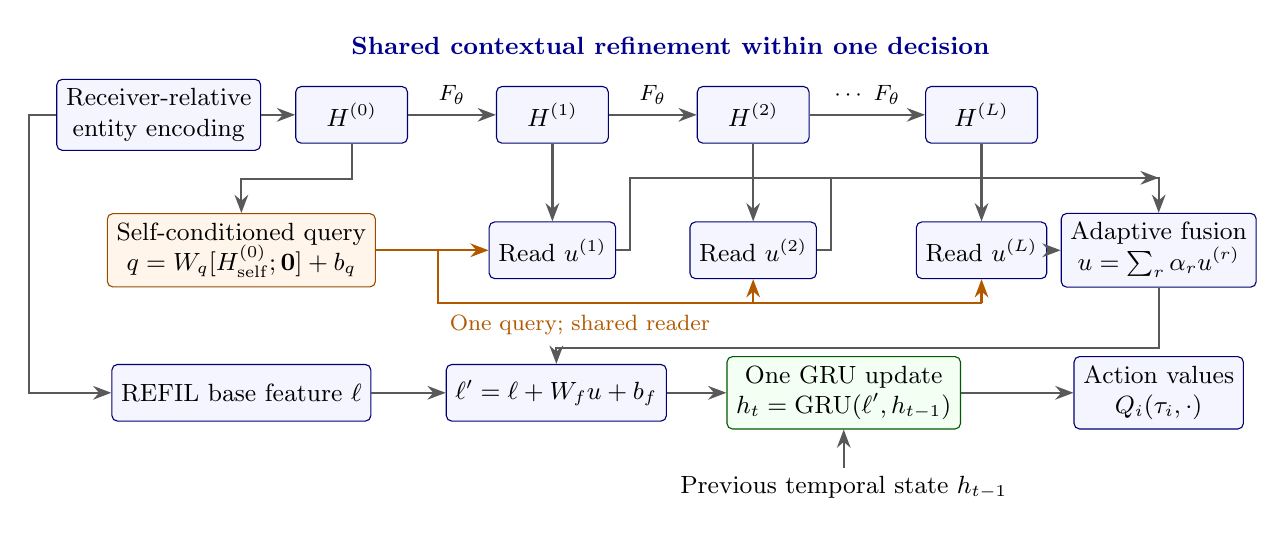
\begin{tikzpicture}[x=1cm,y=1cm,>=Stealth,
 box/.style={draw=blue!45!black,rounded corners=2pt,fill=blue!4,align=center,font=\small,minimum height=.72cm},
 smallbox/.style={box,minimum width=1.42cm},
 flow/.style={->,thick,draw=black!65},
 every node/.style={font=\small}]
\node[box,minimum width=2.1cm] (obs) at (0,0) {Receiver-relative\\entity encoding};
\node[smallbox] (h0) at (2.45,0) {$H^{(0)}$};
\node[smallbox] (h1) at (5.00,0) {$H^{(1)}$};
\node[smallbox] (h2) at (7.55,0) {$H^{(2)}$};
\node[smallbox] (hl) at (10.45,0) {$H^{(L)}$};
\draw[flow] (obs) -- (h0);
\draw[flow] (h0) -- node[above,font=\footnotesize] {$F_\theta$} (h1);
\draw[flow] (h1) -- node[above,font=\footnotesize] {$F_\theta$} (h2);
\draw[flow] (h2) -- node[above,font=\footnotesize] {$\cdots\ F_\theta$} (hl);
\node[font=\small\bfseries,text=blue!55!black] at (6.5,.88) {Shared contextual refinement within one decision};
\node[box,fill=orange!8,draw=orange!60!black,minimum width=2.1cm] (query) at (1.05,-1.72) {Self-conditioned query\\$q=W_q[H^{(0)}_{\mathrm{self}};\mathbf 0]+b_q$};
\node[smallbox] (u1) at (5,-1.72) {Read $u^{(1)}$};
\node[smallbox] (u2) at (7.55,-1.72) {Read $u^{(2)}$};
\node[smallbox] (ul) at (10.45,-1.72) {Read $u^{(L)}$};
\draw[flow] (h0.south) -- ++(0,-.45) -| (query.north);
\draw[flow] (h1) -- (u1);
\draw[flow] (h2) -- (u2);
\draw[flow] (hl) -- (ul);
\draw[flow,draw=orange!70!black] (query.east) -- (u1.west);
\draw[draw=orange!70!black,thick] (3.55,-1.72) -- (3.55,-2.39) -- (10.45,-2.39);
\draw[flow,draw=orange!70!black] (7.55,-2.39) -- (u2.south);
\draw[flow,draw=orange!70!black] (10.45,-2.39) -- (ul.south);
\node[font=\footnotesize,text=orange!70!black] at (5.35,-2.67) {One query; shared reader};
\node[box,minimum width=2.05cm] (fusion) at (12.70,-1.72) {Adaptive fusion\\$u=\sum_r\alpha_r u^{(r)}$};
\draw[flow] (ul) -- (fusion);
\draw[flow] (u1.east) -- ++(.18,0) |- (12.7,-.8) -- (fusion.north);
\draw[flow] (u2.east) -- ++(.18,0) |- (12.7,-.8);
\node[box,minimum width=2.5cm] (base) at (1.05,-3.53) {REFIL base feature $\ell$};
\node[box,minimum width=2.0cm] (res) at (5.05,-3.53) {$\ell'=\ell+W_f u+b_f$};
\node[box,fill=green!5,draw=green!35!black,minimum width=2cm] (gru) at (8.7,-3.53) {One GRU update\\$h_t=\operatorname{GRU}(\ell',h_{t-1})$};
\node[box,minimum width=1.8cm] (qval) at (12.7,-3.53) {Action values\\$Q_i(\tau_i,\cdot)$};
\draw[flow] (obs.west) -- (-1.65,0) |- (base.west);
\draw[flow] (base) -- (res);
\draw[flow] (fusion.south) -- ++(0,-.18) |- (5.05,-2.96) -- (res.north);
\draw[flow] (res) -- (gru);
\draw[flow] (gru) -- (qval);
\node at (8.7,-4.73) {Previous temporal state $h_{t-1}$};
\draw[flow] (8.7,-4.48) -- (gru.south);
\end{tikzpicture}

\caption{LEAF at one defender decision. Receiver-relative entity tokens undergo $L$ applications of a shared contextual-update block. The same self-conditioned query reads each intermediate workspace; learned weights fuse the reads. The result augments the REFIL base feature before one GRU update. Previous memory enters the GRU; its query-input component is zero. LEAF uses no explicit typed-count injection. Training samples $L\in\{1,2,3,4\}$; standard evaluation fixes $L=4$. A new observation initializes the next workspace.}
\label{fig:framework}
\end{figure*}
\section{Looped Entity Attention Fusion}
\label{sec:method}
LEAF repeatedly updates a receiver-relative entity set with one shared attention block, reads every intermediate set using the defender's current self representation, and fuses the reads before updating the recurrent utility network. Figure~\ref{fig:framework} gives the complete information flow.

\subsection{Receiver-Relative Entity Workspace}
At time $t$, defender $i$ receives an entity matrix $X_{i,t}$ and a mask $m_{i,t,e}\in\{0,1\}$, with one denoting a permitted key row. The main branch uses the public entities, while imagined branches impose their additional partition masks. Other entities are encoded relative to defender $i$; its self row retains absolute features. Inputs contain normalized planar positions and velocities, alive/health information, target damage, entity type, and previous-action features. A shared encoder gives entity embeddings $e_{i,t,e}$ and the REFIL feature $\ell_{i,t}$.

The LEAF workspace has width $d=64$. On valid rows its initial representation is
\begin{equation}
 H^{(0)}_{i,t,e}=W_g e_{i,t,e}+b_g.
 \label{eq:workspace}
\end{equation}
The projected self token is retained for query construction under the branch convention, and entity interactions use the permitted-key mask. Excluded rows have no key contribution and are zeroed after each shared update. Each defender thus has a receiver-relative workspace, with common network parameters across defenders and branches. A new observation initializes a new workspace.

The evaluated LEAF configuration disables explicit typed-count injection. Population changes are represented through the observed entity set and its mask. The current observation supplies the reader query; temporal context remains in the downstream recurrent utility network.

\subsection{Repeated Contextual Entity Updates}
Suppressing defender, time, and branch indices, one round applies
\begin{align}
 J^{(r)}&=\operatorname{LN}_a(H^{(r-1)}),\nonumber\\
 \widetilde H^{(r)}&=H^{(r-1)}
       +\operatorname{MHA}_{\theta}(J^{(r)},H^{(r-1)},H^{(r-1)};m),\nonumber\\
 H^{(r)}&=\operatorname{Mask}_{m}\!\left[\widetilde H^{(r)}
       +\operatorname{FFN}_{\theta}
                  (\operatorname{LN}_f(\widetilde H^{(r)}))\right].
 \label{eq:loop}
\end{align}
Here $\operatorname{LN}$ denotes rowwise layer normalization, $\operatorname{MHA}(Q,K,V;m)$ is masked multihead attention, and $\operatorname{Mask}_m$ zeros excluded rows. An empty permitted-key set returns a zero attention aggregate. The same update parameters are reused for $r=1,\ldots,L$. Keys and values at round $r$ are the representations from round $r-1$, so the operator acts on the context produced by its preceding application.

Within the permitted set, attention connects every valid entity to every other valid entity from the first round onward. Later rounds therefore refine already contextualized features. Entity rows retain their identities, and every intermediate set $H^{(1)},\ldots,H^{(L)}$ remains available to the reader. This organization follows shared relational processing~\cite{zambaldi2019relational,dehghani2019universal} and gives the decision stage access to several stages of that processing. The anchored-key/value comparator ARR instead supplies $H^{(0)}$ as keys and values at each update.

\subsection{Self-Conditioned Reading and Temporal Decision}
The receiver constructs one query from its initial self token. The previous-memory input to this query is fixed to zero:
\begin{align}
 q_{i,t}&=W_q[H^{(0)}_{i,t,\mathrm{self}};
                    \mathbf 0]+b_q,\nonumber\\
 u_{i,t}^{(r)}&=\operatorname{MHA}_{\mathrm{read}}
                  (q_{i,t},H_{i,t}^{(r)},H_{i,t}^{(r)};m_{i,t}).
 \label{eq:read}
\end{align}
The readout $u_{i,t}^{(r)}\in\mathbb R^{64}$ summarizes round $r$ for defender $i$. The same query and reader parameters are used for every round at the current decision. Each read attends directly to its corresponding entity set. Thus the reader depends on the current receiver state. This is the saved \texttt{regir\_nomem} configuration (NoMem), denoted LEAF throughout this paper. It retains temporal recurrence through the GRU in Eq.~\eqref{eq:decision}. The separately trained memory-query comparison replaces $\mathbf 0$ in Eq.~\eqref{eq:read} with $\operatorname{sg}(h_{i,t-1})$, where $\operatorname{sg}$ preserves the forward value and stops the gradient through that query-input copy. The GRU's temporal recurrence remains trainable in both designs.

A shared scalar scoring map assigns weights to the available reads:
\begin{equation}
 \alpha_{i,t}^{(r)}=
 \frac{\exp(w_s^\top u_{i,t}^{(r)}+b_s)}
 {\sum_{j=1}^{L}\exp(w_s^\top u_{i,t}^{(j)}+b_s)},\qquad
 u_{i,t}=\sum_{r=1}^{L}\alpha_{i,t}^{(r)}u_{i,t}^{(r)}.
 \label{eq:fusion}
\end{equation}
These nonnegative weights sum to one and are recomputed from the reads at each decision. Entity attention within a round determines what the defender reads, and cross-round fusion determines how those summaries contribute to its decision feature. Both depend on the receiver through its self representation. Preserving intermediate representations provides access across processing depth~\cite{xu2018jk}. This adaptive weighting does not halt the shared updates or select an execution depth; all $L$ rounds are computed.

The fused read augments the REFIL feature through a residual projection:
\begin{align}
 \ell'_{i,t}&=\ell_{i,t}+W_f u_{i,t}+b_f,\nonumber\\
 h_{i,t}&=\operatorname{GRU}(\ell'_{i,t},h_{i,t-1}),\nonumber\\
 Q_i(\tau_{i,t},\cdot)&=W_o h_{i,t}+b_o.
 \label{eq:decision}
\end{align}
The projection $W_fu+b_f$ is initialized to zero, so learning starts from the original feature path and jointly adapts both paths thereafter. Each branch updates the GRU once per defender decision at a physical time step. Its hidden state persists to the next observation, while the entity workspace is rebuilt from that observation. Thus $r$ indexes repeated computation at one decision and $t$ indexes physical evolution. All rounds are computed before fusion; small fusion weights affect information use while the chosen depth $L$ determines the computation performed.



\subsection{Local Sensitivity to Later Reads}
The fusion rule permits an exact decomposition at a fixed decision. Suppress receiver and time indices, and let $u_{[k]}$ denote the fused read when $k$ rounds are executed with the same entities, previous actions, and incoming GRU state. The first two workspaces and reads are identical in two- and four-round execution. Using the four-round weights, set $\epsilon=\alpha^{(3)}+\alpha^{(4)}$ and, for $0<\epsilon<1$, define
\begin{align}
 \mu_{\mathrm E}&=
 \frac{\alpha^{(1)}u^{(1)}+\alpha^{(2)}u^{(2)}}{1-\epsilon},\nonumber\\
 \mu_{\mathrm L}&=
 \frac{\alpha^{(3)}u^{(3)}+\alpha^{(4)}u^{(4)}}{\epsilon}.
 \label{eq:early-late-reads}
\end{align}
Because the scoring map is shared, normalizing only the first two scores gives $u_{[2]}=\mu_{\mathrm E}$. Hence
\begin{align}
 u_{[4]}-u_{[2]}&=\epsilon(\mu_{\mathrm L}-\mu_{\mathrm E}),\nonumber\\
 \ell'_{[4]}-\ell'_{[2]}&=
 \epsilon W_f(\mu_{\mathrm L}-\mu_{\mathrm E}).
 \label{eq:depth-perturbation}
\end{align}
The projection bias cancels. Small late-read weight alone therefore does not bound the feature perturbation: the separation of the read summaries and the learned projection also matter.

Let $Q^{[k]}$ be the resulting action-value vector after one GRU update from the same incoming state. For the unique four-round greedy action $a^\star$, define its legal-action margin $g=Q^{[4]}_{a^\star}-\max_{a\in\mathcal U\setminus\{a^\star\}}Q^{[4]}_a$ and $\delta Q=Q^{[2]}-Q^{[4]}$. A sufficient condition for retaining that action is
\begin{equation}
 g>2\|\delta Q\|_\infty.
 \label{eq:greedy-stability}
\end{equation}
Indeed, every perturbed action gap is at least $g-2\|\delta Q\|_\infty$. This condition is sufficient rather than necessary. It explains local action sensitivity at a recorded decision; it gives no closed-loop reward guarantee once actions change subsequent states and recurrent histories.

\subsection{Learning Across Processing Depths}
Collection samples $L$ uniformly from $\{1,2,3,4\}$ and holds it fixed for an episode. Replay independently samples one depth per training batch and uses that depth for the online main and imagined branches and the target network. At depth one, the shared update directly supplies the value objective. At larger depths, its output also becomes the input to subsequent applications. Consequently, the same parameters learn through both short decision paths and longer sequences of contextual updates. Standard deployment fixes $L=4$.

Learning retains the shared potential-shaped reward used by the REFIL host:
\begin{align}
 \widetilde r_t&=-\Delta D_t+\gamma\Phi(s_{t+1})-\Phi(s_t),\nonumber\\
 \Phi(s)&=-\sum_{j\in\mathcal B_{\mathrm{alive}}}
 \operatorname{clip}\!\left(1-\frac{\min_{k\in\mathcal T}\|p_j-p_k\|}{4000},0,1\right),
 \label{eq:shaping}
\end{align}
where $p_j$ and $p_k$ are attacker and target positions, $\operatorname{clip}(a,0,1)$ truncates $a$ to $[0,1]$, and $\gamma=0.99$. This potential supplies a dense proximity signal during learning. Evaluation reports the unshaped episode reward $R=-D$ in Eq.~\eqref{eq:damage}, for which larger values indicate better protection.

Natural termination zeros the bootstrap; time-limit transitions retain a valid successor. If the last defender disappears, the discounted reward tail from the remaining physical simulation is folded into the final defender decision transition. Let $\bar r_t$ be the resulting replay reward and $b_t$ its bootstrap multiplier, with $b_t=\gamma$ for an ordinary nonterminal transition and $b_t=0$ after natural termination. Online utilities select legal greedy successor actions $\boldsymbol a^*_{t+1}$, and the target network evaluates
\begin{equation}
 y_t=\bar r_t+b_t
 Q^-_{\mathrm{tot}}(x_{t+1},\boldsymbol a^*_{t+1}).
 \label{eq:td-target}
\end{equation}
With $Q_{\mathrm{main},b,t}=Q_{\mathrm{tot},b,t}$ and imagined value $Q_{\mathrm{aux},b,t}$, the loss on a replay minibatch indexed by sequence $b$ and step $t$ is
\begin{align}
 \mathcal L&=(1-\lambda)\mathcal L_{\mathrm{main}}
                  +\lambda\mathcal L_{\mathrm{aux}},\qquad\lambda=0.5,\nonumber\\
 \mathcal L_k&=\frac{\sum_{b,t} v_{b,t}(Q_{k,b,t}-y_{b,t})^2}
 {\sum_{b,t}v_{b,t}},
 \quad k\in\{\mathrm{main},\mathrm{aux}\},
 \label{eq:td-loss}
\end{align}
where $v_{b,t}$ marks valid transitions and $y_{b,t}$ is detached during optimization. Both losses normalize over the minibatch's valid transitions. The main and imagined branches reconstruct their masked histories with shared parameters. Deployment uses the main branch. Algorithm~\ref{alg:leaf} summarizes one decision.

\begin{algorithm}[!t]
\caption{LEAF at one defender decision}
\label{alg:leaf}
\begin{algorithmic}[1]
\Require Entity features $X_{i,t}$, mask $m_{i,t}$, memory $h_{i,t-1}$, depth $L$
\State Encode entities and compute base feature $\ell_{i,t}$
\State Initialize workspace and self-conditioned query $q_{i,t}$
\For{$r=1,\ldots,L$}
\State Update $H_{i,t}^{(r)}$ with the shared block, Eq.~\eqref{eq:loop}
\State Read $u_{i,t}^{(r)}$ with $q_{i,t}$, Eq.~\eqref{eq:read}
\EndFor
\State Fuse reads and add the residual to $\ell_{i,t}$
\State Update the GRU once and compute action values
\State \Return $\arg\max_{a\in\mathcal U_{i,t}}Q_i(\tau_{i,t},a)$ and $h_{i,t}$
\end{algorithmic}
\end{algorithm}

\subsection{Execution Properties}
Shared rowwise maps and masked attention preserve entity identities throughout refinement and support variable-size sets. Permuting the non-self entities together with their masks permutes every intermediate workspace while leaving the receiver query and the resulting action values unchanged. This consistency follows through the recurrent policy from identical initial memory. It establishes ordering consistency, while reward under a changed population remains an empirical question.

For $M$ padded entity slots and width $d$, dense refinement costs $O(L(M^2d+Md^2))$ per receiver. Parameters are shared across rounds, while computation grows with the chosen unfolding depth. The implementation forms receiver-relative views for live defenders. Parameter sharing limits growth with depth but does not remove this computational cost. The present final-checkpoint evaluation fixes the execution depth; no real-time deployment claim is inferred from the asymptotic expression.

\section{Experimental Evaluation}
\label{sec:results}
% Numerical source: main0928/had/aggregates.json, paper1007.
% R=-D. SD is sample SD (ddof=1); learning-method unit is training seed.
% The optional full-variant macro is placed by main.tex in its existing appendix.

\newcommand{\HadMainTable}{%
\begin{table*}[!t]
\centering\footnotesize
\setlength{\tabcolsep}{5pt}
\caption{Formal HAD comparison: mean $\pm$ sample SD. Reward $R=-D$ is higher-is-better; friendly-collision mortality $C$ is lower-is-better. Each learned method has three training seeds and 300 common scenes per configuration. Bold marks the best group mean for each metric.}
\label{tab:had-main}
\begin{tabular*}{\textwidth}{@{\extracolsep{\fill}}llrrrr@{}}
\toprule
Method & Metric & ID & $K$-OOD & $N$-OOD & Joint OOD \\
\midrule
\textbf{LEAF} & $R\uparrow$ & $\mathbf{-0.405\pm0.097}$ & $\mathbf{-0.996\pm0.233}$ & $\mathbf{-0.575\pm0.235}$ & $\mathbf{-1.097\pm0.105}$ \\
 & $C\downarrow$ (\%) & $\mathbf{1.33\pm0.45}$ & $\mathbf{1.70\pm0.62}$ & $6.29\pm1.32$ & $4.97\pm1.26$ \\
\addlinespace[2pt]
REFIL & $R\uparrow$ & $-0.715\pm0.049$ & $-1.796\pm0.304$ & $-2.209\pm0.277$ & $-3.308\pm0.303$ \\
 & $C\downarrow$ (\%) & $2.97\pm0.42$ & $4.71\pm0.67$ & $12.86\pm2.14$ & $10.34\pm1.69$ \\
\addlinespace[2pt]
QMIX-Atten & $R\uparrow$ & $-2.318\pm1.431$ & $-5.009\pm2.497$ & $-5.139\pm3.111$ & $-7.415\pm3.970$ \\
 & $C\downarrow$ (\%) & $10.82\pm9.56$ & $12.42\pm9.75$ & $16.38\pm5.43$ & $15.37\pm7.34$ \\
\addlinespace[2pt]
DCG & $R\uparrow$ & $-2.028\pm0.437$ & $-5.839\pm1.920$ & $-5.021\pm2.658$ & $-8.092\pm3.909$ \\
 & $C\downarrow$ (\%) & $9.05\pm3.36$ & $14.97\pm4.68$ & $19.70\pm8.52$ & $19.26\pm10.20$ \\
\addlinespace[2pt]
SPECTra & $R\uparrow$ & $-2.662\pm0.070$ & $-6.933\pm0.670$ & $-6.455\pm1.403$ & $-11.184\pm0.352$ \\
 & $C\downarrow$ (\%) & $13.06\pm0.75$ & $20.71\pm1.60$ & $28.92\pm1.54$ & $31.25\pm1.63$ \\
\addlinespace[2pt]
ALMA & $R\uparrow$ & $-1.326\pm0.193$ & $-3.022\pm0.344$ & $-3.605\pm0.742$ & $-5.375\pm1.036$ \\
 & $C\downarrow$ (\%) & $7.42\pm1.13$ & $9.05\pm1.66$ & $18.42\pm3.84$ & $15.92\pm3.86$ \\
\addlinespace[2pt]
Rule$^{\dagger}$ & $R\uparrow$ & $-1.462\pm0.717$ & $-3.212\pm1.126$ & $-1.545\pm0.881$ & $-3.060\pm0.976$ \\
 & $C\downarrow$ (\%) & $1.98\pm4.47$ & $2.70\pm3.57$ & $\mathbf{5.70\pm3.30}$ & $\mathbf{4.48\pm2.44}$ \\
\bottomrule
\end{tabular*}
\par\vspace{2pt}\parbox{\textwidth}{\footnotesize
$\dagger$ Rule has no training seeds. Its SD is across the 300 scene seeds, after averaging configurations within each scene. All other SDs measure training-seed variation. Collision SDs are percentage points.}
\end{table*}}

\newcommand{\HadCoreAblationTable}{%
\begin{table*}[!t]
\centering\footnotesize
\setlength{\tabcolsep}{5pt}
\caption{Core design references on the formal HAD matrix: absolute reward $R=-D$ and friendly-collision mortality $C$, mean $\pm$ sample SD across three training seeds. Each configuration uses 300 common scenes. Bold marks the best mean among these five methods. SG denotes + Memory query; NoREFIL, R0, and R1 retain historical-query inputs.}
\label{tab:had-core-ablation}
\begin{tabular*}{\textwidth}{@{\extracolsep{\fill}}llrrrr@{}}
\toprule
Method & Metric & ID & $K$-OOD & $N$-OOD & Joint OOD \\
\midrule
\textbf{LEAF} & $R\uparrow$ & $\mathbf{-0.405\pm0.097}$ & $\mathbf{-0.996\pm0.233}$ & $\mathbf{-0.575\pm0.235}$ & $\mathbf{-1.097\pm0.105}$ \\
 & $C\downarrow$ (\%) & $\mathbf{1.33\pm0.45}$ & $\mathbf{1.70\pm0.62}$ & $\mathbf{6.29\pm1.32}$ & $\mathbf{4.97\pm1.26}$ \\
\addlinespace[2pt]
SG (+ Memory query) & $R\uparrow$ & $-0.527\pm0.227$ & $-1.529\pm0.734$ & $-0.998\pm0.621$ & $-1.946\pm1.229$ \\
 & $C\downarrow$ (\%) & $1.66\pm0.86$ & $2.59\pm1.78$ & $8.57\pm4.41$ & $6.65\pm4.16$ \\
\addlinespace[2pt]
NoREFIL & $R\uparrow$ & $-0.510\pm0.138$ & $-1.768\pm0.621$ & $-1.263\pm0.653$ & $-2.319\pm0.889$ \\
 & $C\downarrow$ (\%) & $2.23\pm0.77$ & $3.67\pm1.65$ & $10.71\pm3.98$ & $8.76\pm3.14$ \\
\addlinespace[2pt]
R0 & $R\uparrow$ & $-0.928\pm0.210$ & $-1.958\pm0.457$ & $-2.020\pm0.446$ & $-3.196\pm0.687$ \\
 & $C\downarrow$ (\%) & $3.34\pm1.66$ & $4.46\pm2.10$ & $11.16\pm1.81$ & $9.17\pm2.18$ \\
\addlinespace[2pt]
1-round (R1) & $R\uparrow$ & $-0.609\pm0.272$ & $-1.203\pm0.402$ & $-1.355\pm0.884$ & $-2.157\pm1.006$ \\
 & $C\downarrow$ (\%) & $1.57\pm0.15$ & $2.08\pm0.32$ & $8.35\pm3.16$ & $6.56\pm2.37$ \\
\bottomrule
\end{tabular*}
\par\vspace{2pt}\parbox{\textwidth}{\footnotesize
Groups weight configurations equally within each training seed. All SDs measure training-seed variation; collision SDs are percentage points. These are absolute results for complete trained designs, with the paired design questions explained in the text.}
\end{table*}}

\newcommand{\HadFullVariantTable}{%
\begin{table*}[!t]
\centering\footnotesize
\setlength{\tabcolsep}{4pt}
\caption{All ten completed main0928 design variants on the same formal matrix: reward mean $\pm$ sample SD across three training seeds. These results retain the context in which LEAF was selected. Comparison variants beyond + Memory query also change architecture or training/execution choices.}
\label{tab:had-full-variants}
\begin{tabular*}{\textwidth}{@{\extracolsep{\fill}}lrrrr@{}}
\toprule
Method & ID & $K$-OOD & $N$-OOD & Joint OOD \\
\midrule
\textbf{LEAF} & $-0.405\pm0.097$ & $-0.996\pm0.233$ & $-0.575\pm0.235$ & $-1.097\pm0.105$ \\
+ Memory query & $-0.527\pm0.227$ & $-1.529\pm0.734$ & $-0.998\pm0.621$ & $-1.946\pm1.229$ \\
NoREFIL & $-0.510\pm0.138$ & $-1.768\pm0.621$ & $-1.263\pm0.653$ & $-2.319\pm0.889$ \\
R0 & $-0.928\pm0.210$ & $-1.958\pm0.457$ & $-2.020\pm0.446$ & $-3.196\pm0.687$ \\
1-round & $-0.609\pm0.272$ & $-1.203\pm0.402$ & $-1.355\pm0.884$ & $-2.157\pm1.006$ \\
Last & $-0.434\pm0.083$ & $-1.020\pm0.100$ & $-0.652\pm0.160$ & $-1.269\pm0.202$ \\
Fixed4 & $-0.407\pm0.204$ & $-1.004\pm0.665$ & $-0.659\pm0.184$ & $-1.265\pm0.230$ \\
ARR & $-0.469\pm0.091$ & $-1.221\pm0.344$ & $-1.778\pm1.292$ & $-2.370\pm1.164$ \\
Untied4 & $-0.476\pm0.183$ & $-1.127\pm0.157$ & $-0.543\pm0.156$ & $-1.232\pm0.253$ \\
Looped + count & $-0.596\pm0.145$ & $-1.301\pm0.427$ & $-1.075\pm0.449$ & $-1.685\pm0.844$ \\
\bottomrule
\end{tabular*}
\end{table*}}


\noindent\textbf{Setup and statistics.}
We evaluate HAD target protection against a fixed reactive--rush attacker, using public physical entity states and a horizon of 100 environment steps. Training samples balanced teams $N_R=N_B=N\in\{4,6,8,10\}$ and target counts $K\in\{1,2,3\}$. Each learned method has three training seeds and a nominal budget of $10^6$ physical environment steps per seed. LEAF retains the REFIL host and downstream GRU, uses a self-conditioned relation query without previous GRU state, disables explicit count injection, samples one through four relation rounds during training, and executes four rounds for formal evaluation. Hidden width is 64, with four attention heads, learning rate $5\times10^{-4}$, discount 0.99, batch size 32, and replay capacity 5000.

Frozen final checkpoints are evaluated on 24 configurations, with 300 common scene seeds (9000--9299) per configuration. ID comprises $(4,4,2)$, $(6,6,2)$, $(8,8,2)$, and $(10,10,3)$. $K$-OOD uses $(10,10,K)$ for $K\in\{4,6,9,12\}$; $N$-OOD uses $(N,N,2)$ for $N\in\{15,20,25,30,40,50\}$. Joint OOD combines $N\in\{15,20,30\}$ with $K\in\{4,6\}$ and adds $(30,30,9)$ and $(30,30,12)$. Supporting configurations are $(5,5,2)$ and $(10,10,2)$. The learned baselines are REFIL, QMIX-Atten, DCG, SPECTra, and ALMA; Rule is a fixed policy. Historical baseline checkpoints and their evaluation slices are reused with their recorded identities and interaction budgets.

The primary metric is unshaped episode reward $R=-D$, with higher values indicating better protection. The second metric is friendly-collision mortality,
\begin{equation}
 C=\frac{\text{defenders killed by friendly collision}}{N_R},
\end{equation}
with lower values preferred. Each training seed first averages the 300 scenes within a configuration and then weights configurations equally within a group. We report mean $\pm$ sample standard deviation (SD) across the three trained models. For Rule, configurations are averaged within each common scene seed before computing SD across 300 scene seeds. These SDs describe different sources of variation and are not confidence intervals~\cite{agarwal2021rliable}.

Training validation uses 50 checkpoints and the same four ID configurations, with 25 fixed scenes per configuration in seed blocks spanning 9500--9599. Curves align evaluation indices, average configurations within each training seed, and show the three-seed mean and sample SD at the mean recorded environment step count, without smoothing. Validation scenes differ from the 300-scene formal evaluation pool, so the last curve point need not equal the ID value in the formal tables.

\subsection{Comparison Across Deployment Populations}
\label{subsec:comparison}
Table~\ref{tab:had-main} shows the highest group mean reward for LEAF among the six learned methods and Rule in all four groups. Relative to REFIL, its reward improves by 0.310, 0.800, 1.635, and 2.211 in ID, $K$-OOD, $N$-OOD, and Joint OOD. Each improvement holds in all three corresponding training-seed comparisons. Figure~\ref{fig:had-generalization} shows validation during training separately from target-count, team-size, and joint transfer of frozen final checkpoints.

At validation checkpoint 10 (approximately $0.2$ million steps), LEAF has reward $-2.046\pm0.028$ versus REFIL's $-4.429\pm0.284$. At checkpoint 50, the values are $-0.373\pm0.066$ and $-0.738\pm0.122$. These observations describe the recorded ID learning trajectories; they do not establish an improvement for every checkpoint or a general sample-efficiency claim.

LEAF has lower mean collision mortality than every learned baseline in each group. Rule has lower mortality in $N$-OOD (5.70\% versus 6.29\%) and Joint OOD (4.48\% versus 4.97\%), despite lower reward. Minimizing friendly losses alone therefore does not explain target protection.

\HadMainTable

\begin{figure*}[!t]
\centering
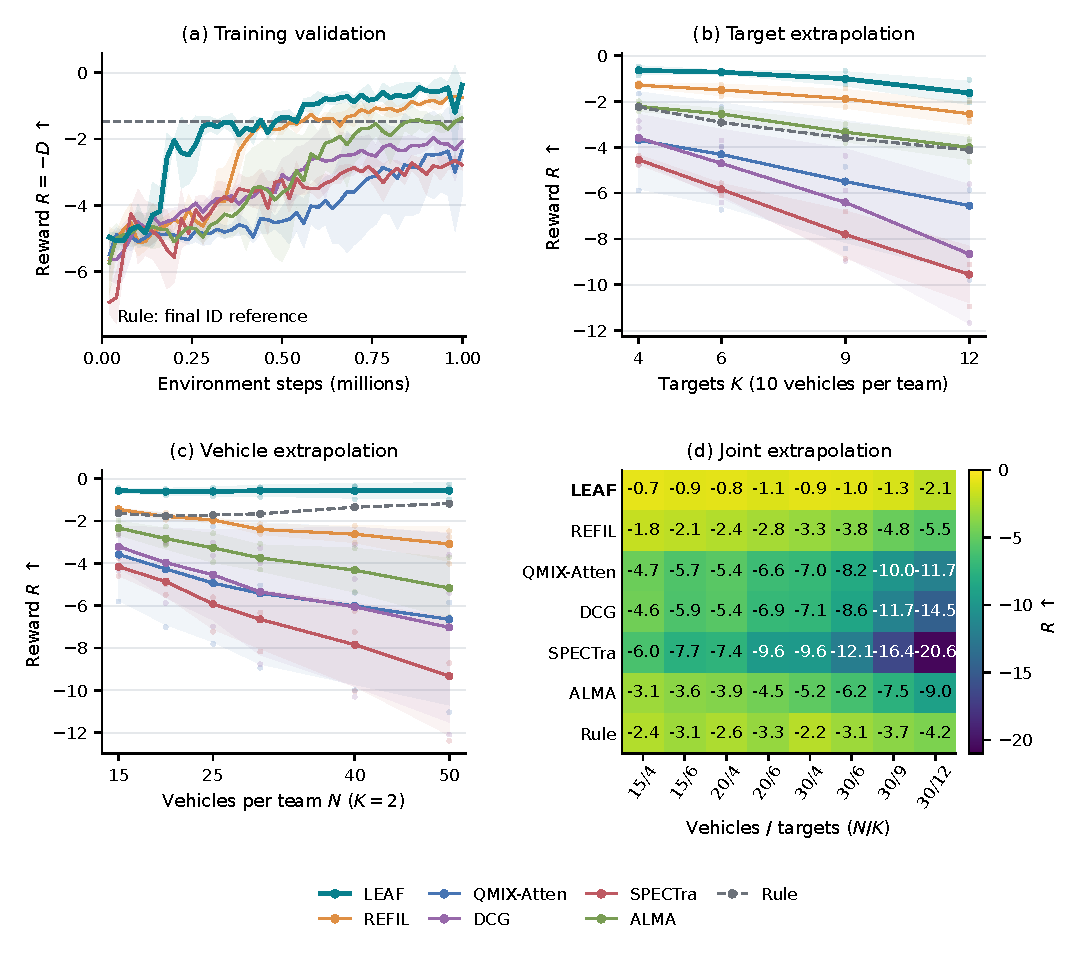
\includegraphics[width=\textwidth]{figures/fig_had_generalization.pdf}
\caption{Learning and formal generalization. (a) Fifty native validation checkpoints for LEAF and the five learned baselines, plotted at actual mean environment steps without smoothing; bands show one training-seed sample SD. Validation uses fixed scene seeds 9500--9599; Rule is a formal final-ID reference. (b)--(c) Target-count and team-size transfer retain seed points and SD bands. (d) All eight Joint OOD configurations share a linear reward scale. Learning-record sources are described in Appendix~\ref{app:learning-source}.}
\label{fig:had-generalization}
\end{figure*}

\subsection{Ablation and Design Comparisons}
\label{subsec:ablation}
Table~\ref{tab:had-core-ablation} reports absolute reward and collision mortality for the five core design references across all four groups. Figure~\ref{fig:had-ablation} complements those endpoints with validation during training and transfer along the target, vehicle, and joint population axes. The design study addresses three paired questions. First, does contextual entity processing help before reading? Within the historical-query branch, R0 reads the original entity representations, whereas 1-round (R1) performs one contextual update. R1 improves mean reward by 0.319, 0.755, 0.665, and 1.039 across ID, $K$-OOD, $N$-OOD, and Joint OOD, respectively. Two of three seed pairs improve in each group. This comparison supports developing entity context before the readout.

Second, does the relation query need an additional GRU-history input? The closest contrast to LEAF restores detached GRU history in that query, denoted \emph{+ Memory query} (the historical SG variant). Both policies retain downstream recurrence and previous-action input features. Removing GRU history from the query gives LEAF mean reward gains of 0.122, 0.533, 0.424, and 0.849 across the four groups, with agreement in all three ID seeds and two of three seeds per OOD group. This favors self-conditioned reading with temporal memory downstream at the group-mean level. Frozen GRU intervention below examines whether the saved LEAF policy actually depends on that downstream memory.

Third, how does the relational path work with its host? NoREFIL removes the local host, imagination paths, and associated losses while retaining a historical query. Restoring this bundle gives SG higher mean reward in the three extrapolation groups by 0.239, 0.265, and 0.372, with a slight ID decrease of 0.017. This is a whole-architecture contrast; it does not isolate the contribution of any one removed path or loss. Together, the three comparisons examine contextual processing, memory placement, and host integration without treating all variants as single-component deletions from LEAF.

\HadCoreAblationTable

\begin{figure*}[!t]
\centering
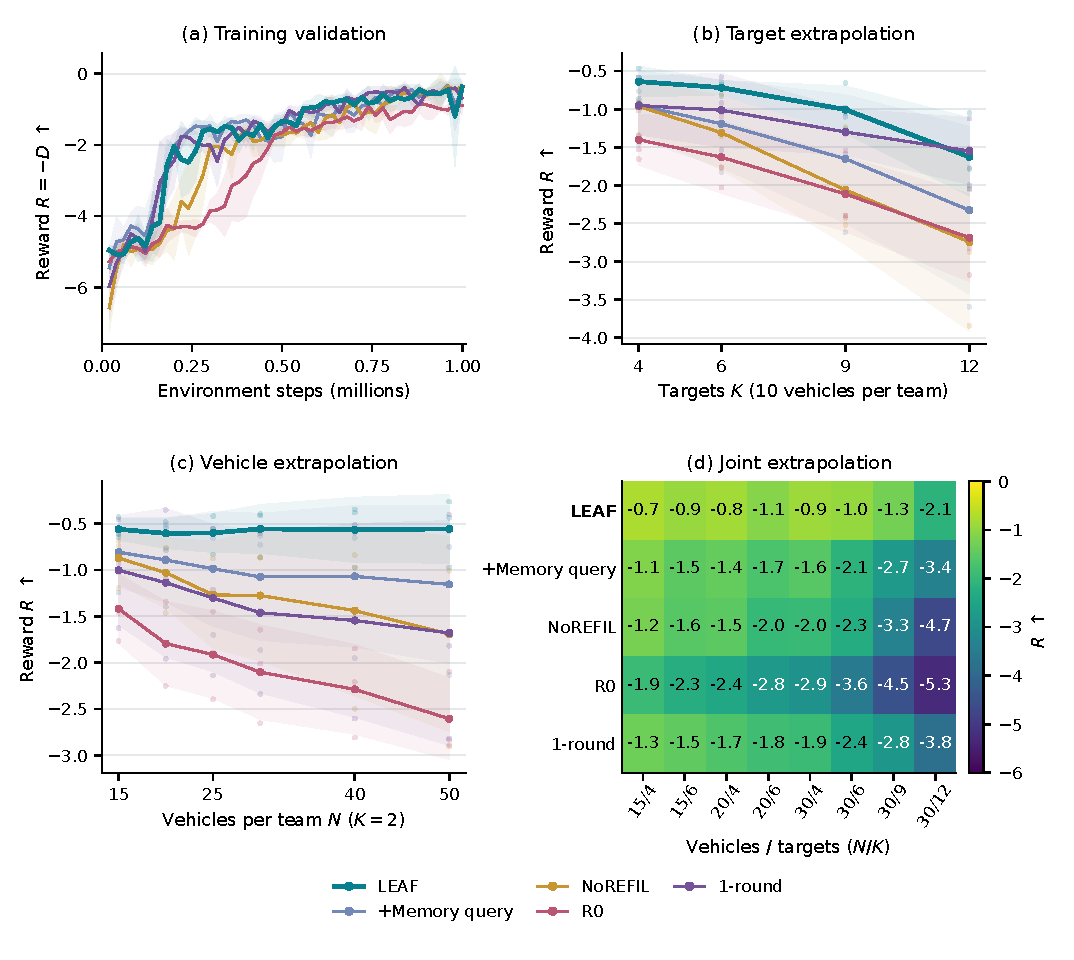
\includegraphics[width=\textwidth]{figures/fig_had_ablation.pdf}
\caption{Validation and population transfer for LEAF, SG (+ Memory query), NoREFIL, R0, and 1-round (R1). (a) Fifty validation checkpoints aligned by evaluation index, with actual mean environment steps on the horizontal axis and mean $\pm$ sample SD across three training seeds; no smoothing is applied. (b)--(c) Absolute reward under target-count and vehicle-count extrapolation, retaining seed points and SD bands. (d) All eight Joint OOD configurations use one linear reward scale, with cell means rounded for display. SG, NoREFIL, R0, and R1 use historical queries. NoREFIL to SG restores the local host, imagination paths, and associated losses together. The text distinguishes the three paired design questions from complete-design comparisons with LEAF and from frozen execution interventions.}
\label{fig:had-ablation}
\end{figure*}

NoREFIL, R0, and R1 are complete-design references when compared directly with LEAF because they also use a historical query. QMIX-Atten and REFIL provide external and host references in Table~\ref{tab:had-main}. A capacity control, REFIL-matched, has 176,393 actor parameters versus LEAF's 175,754 (a 0.36\% difference) and REFIL's 102,025. Its group reward means are $-0.914$, $-2.493$, $-2.269$, and $-4.170$; LEAF improves each in all three seed pairs. This weakens a parameter-count-only explanation, while leaving architecture and optimization differences coupled.

Similar ID validation endpoints do not guarantee similar transfer: NoREFIL's last validation reward is $-0.381\pm0.126$, close to LEAF's $-0.373\pm0.066$, but its formal OOD group means are lower. Group means also do not imply superiority at every configuration: at $(10,10,12)$, R1 has reward $-1.548\pm0.439$ versus LEAF's $-1.625\pm0.515$.

LEAF was selected after inspecting ten completed variants on the formal matrix. Table~\ref{tab:had-full-variants} preserves that selection context. Increasing beyond one round does not improve every group, and learned fusion, depth sampling, and parameter sharing give mixed trained-design results. These choices remain part of the evaluated architecture rather than separate improvement claims. Untied4 has a higher $N$-OOD reward mean than LEAF ($-0.543$ versus $-0.575$); LEAF is higher in the other groups.

\subsection{Mechanism: Looped Context, Fusion, and Memory}
\label{subsec:mechanism}
\noindent\textbf{Protocol.}
Frozen interventions use three registered LEAF final checkpoints at $(10,10,2)$, $(50,50,2)$, and $(30,30,12)$ on common scenes 9000--9009, without weight updates. Eight execution changes examine one or two rounds, reading original tokens $H^{(0)}$ without contextual updates, final-read-only fusion, uniform fusion, fixed mean fusion, zero relation residual, and GRU reset. The $H^{(0)}$ control preserves the self query, read attention, residual projection, local host, and GRU. Residual zeroing removes the complete projection including its bias; GRU reset retains previous-action features.

For fixed fusion, each model's factual fusion weights are averaged over live decisions within each configuration, then equally over the three configurations. These four nonuniform weights replace state-dependent scores at every decision; all four contextual updates and reads remain. This is a diagnostic mean computed on the same scene pool, without reward optimization or a held-out calibration claim.

Closed-loop reward changes are paired with a local standard execution within scene and model seed, averaged over ten scenes, then summarized across three seeds. Same-state forwards separately reuse standard entities, previous actions, and incoming GRU state, restoring factual hidden state, cached values, and random state before the rollout continues. Action-change rates count live defender decisions. The study executed 990 episodes: the original 720, plus 90 standard recaptures and 180 new loop/fusion controls. All 90 recaptures match the earlier local standard in 11 fields. Historical comparison has a narrower agreement range (Appendix~\ref{app:replay}), so these diagnostics do not replace formal performance estimates.

\noindent\textbf{Looped processing builds decision-relevant context.}
Reading $H^{(0)}$ without the loop changes 69.62--72.41\% of same-state greedy actions. Relative to standard LEAF, reward changes by $-7.556\pm1.365$, $-18.962\pm5.828$, and $-32.968\pm8.447$ in the configuration order above; all nine model--configuration means decrease. The R0--R1 trained-design contrast in Section~\ref{subsec:ablation} favors one contextual update, and this direct frozen control establishes that LEAF's learned policy relies on the resulting context. Together they support entity processing before reading. They do not establish that four updates are necessary: two-round reward changes are $-0.273\pm0.047$, $0.001\pm0.205$, and $0.264\pm1.259$, respectively.

\noindent\textbf{Fusion favors early context, with conditional later-read sensitivity.}
The first two rounds receive 98.59--98.91\% of average fusion weight. Forcing the final read, using uniform fusion, or zeroing the relation projection reduces reward in all nine model--configuration means (Fig.~\ref{fig:had-mechanism}). These interventions show reliance on access to the learned intermediate features, but do not alone establish the benefit of state-dependent weights over a fixed shallow preference.

The fixed mean control makes that distinction: it changes 9.88--10.54\% of same-state actions, yet reward changes are $0.006\pm0.109$, $0.092\pm0.121$, and $-0.612\pm0.471$. Its effect is mixed across models at the two $K=2$ configurations, whereas all three models lose reward at $(30,30,12)$. Thus state-dependent fusion has consistent local support in the target-rich case; a broad dynamic-fusion advantage is not established. The strongest shared finding is selective use of early contextual reads.

Later reads still affect a small subset of decisions. Of 48,705 factual live-defender decisions, two-round execution changes 753 actions. Within every model--configuration group, changed decisions have smaller average standard Q margins and larger late-round weights than unchanged decisions. Approximately 78.63\%, 80.88\%, and 78.30\% of changes fall in the lowest-margin decile of their respective groups, averaged equally over model seeds (Fig.~\ref{fig:fusion-sensitivity}). Equation~\eqref{eq:depth-perturbation} relates late weight to the projected feature change; Eq.~\eqref{eq:greedy-stability} explains why small perturbations can matter near an action boundary. Its sufficient condition covers 78.56--83.76\% of decisions, all with unchanged actions. This reconciles shallow weight concentration with local later-read sensitivity, without assigning every changed action a beneficial reward effect.

\noindent\textbf{Temporal memory and protective outcomes complete the account.}
Resetting downstream GRU state changes 58.37--62.90\% of same-state actions and decreases reward in eight of nine model--configuration means; seed 0 at $(30,30,12)$ is the exception. This complements the SG--LEAF comparison: omitting historical input from the query leaves a useful temporal role downstream. At $(50,50,2)$ in the formal 300-scene evaluation, LEAF has collision mortality $11.14\%\pm2.63\%$ versus REFIL's $19.59\%\pm3.69\%$, attacker interception $78.68\%\pm1.39\%$ versus $72.27\%\pm0.77\%$, and any-target-damage incidence $28.11\%\pm15.03\%$ versus $70.56\%\pm7.65\%$. These outcomes associate higher reward with effective protection. A separate common 100-scene arm finds higher geometric pursuit overlap for LEAF ($43.93\%\pm4.20\%$ versus $35.49\%\pm1.50\%$), so uniformly reducing duplicate pursuit is not the explanation. The overlap measure counts attackers pursued by at least two defenders within 1500\,m and a $30^\circ$ velocity cone; it does not label allocation errors.

\begin{figure*}[!t]
\centering
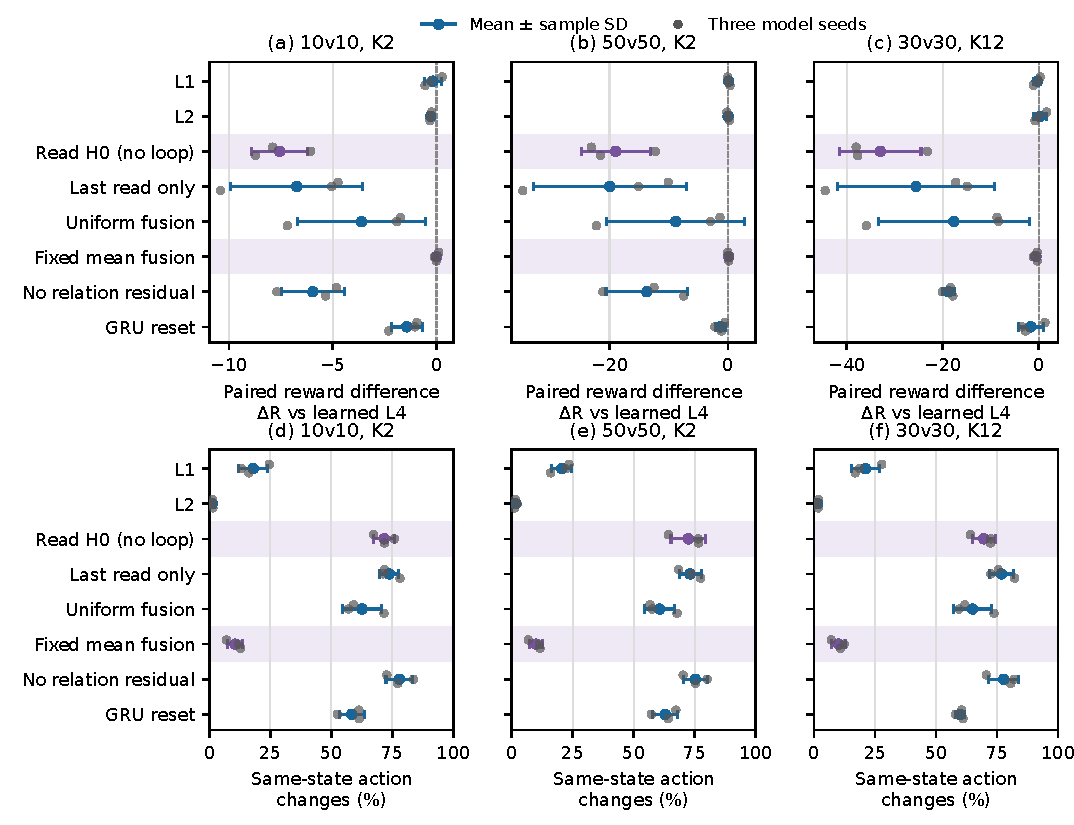
\includegraphics[width=\textwidth]{figures/fig_leaf_final1007_mechanism.pdf}
\caption{Eight frozen-final LEAF interventions on three configurations and ten common scenes per model seed. Top: reward change relative to local standard four-round fusion; positive values favor the intervention. Bottom: same-state greedy-action changes. Points and bars show three-model mean and sample SD; small points retain each model. Shaded loop/fixed-fusion controls use the new runtime, with remaining arms from the original runtime; each is paired with its own local standard (Appendix~\ref{app:replay}). Frozen execution dependence differs from retrained design effects.}
\label{fig:had-mechanism}
\end{figure*}

\begin{figure*}[!t]
\centering
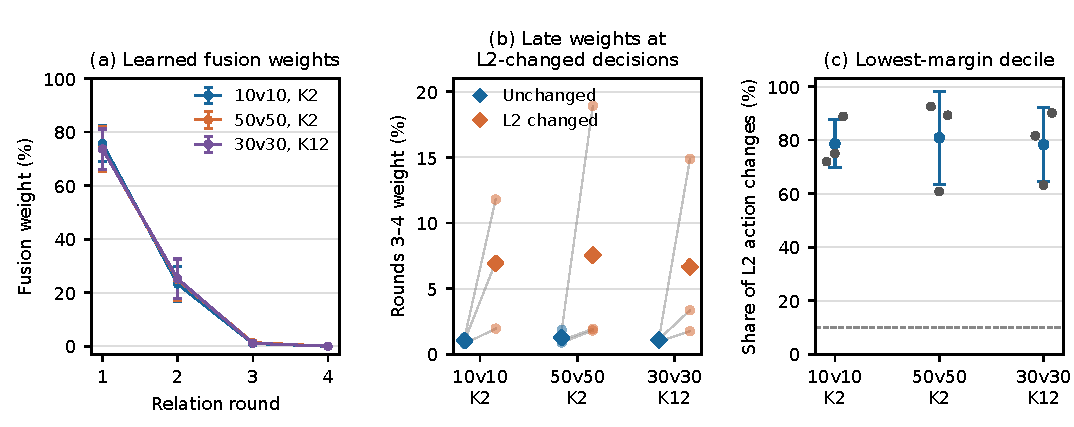
\includegraphics[width=\textwidth]{figures/fig_leaf_fusion_sensitivity.pdf}
\caption{Early-read preference and conditional later-read sensitivity on 90 standard LEAF trajectories. (a) Mean fusion weights with model-seed sample SD. (b) Late-round weight among decisions whose actions change under L2 versus those unchanged: small connected points pair each model; diamonds show the three-model mean. (c) Fraction of L2 action changes in the lowest Q-margin decile within each model and configuration; bars show model-seed SD and the dashed line marks 10\%. These local diagnostics describe decision sensitivity, not the direction of closed-loop reward effects.}
\label{fig:fusion-sensitivity}
\end{figure*}

\subsection{Representative Trajectories}
\label{subsec:trajectories}
Figure~\ref{fig:had-cases} compares LEAF, the five learned baselines, and Rule at $(5,5,2)$ and $(15,15,2)$. The learned policies use registered final checkpoints with training seed 0; both configurations use the preselected scene seed 9000. Initial physical states are identical across all seven methods within each configuration. A common snapshot at physical step 30 shows approach paths and surviving entities, while the adjacent reward plot follows each complete episode to its actual termination.

At 5v5, LEAF, REFIL, and ALMA each finish with reward $-1$, so this scene does not establish a unique LEAF advantage. At 15v15, LEAF prevents target damage and terminates at step 35; REFIL, QMIX-Atten, DCG, SPECTra, ALMA, and Rule receive $-5$, $-6$, $-7$, $-5$, $-1$, and $-1$, respectively. The panels connect movement and interception to the timing of target damage under a shared initial layout. These illustrative cases do not replace the 300-scene population statistics. Eleven of the fourteen local replays match all archived comparison fields; the remaining differences are retained in Appendix~\ref{app:replay}.

\begin{figure*}[!t]
\centering
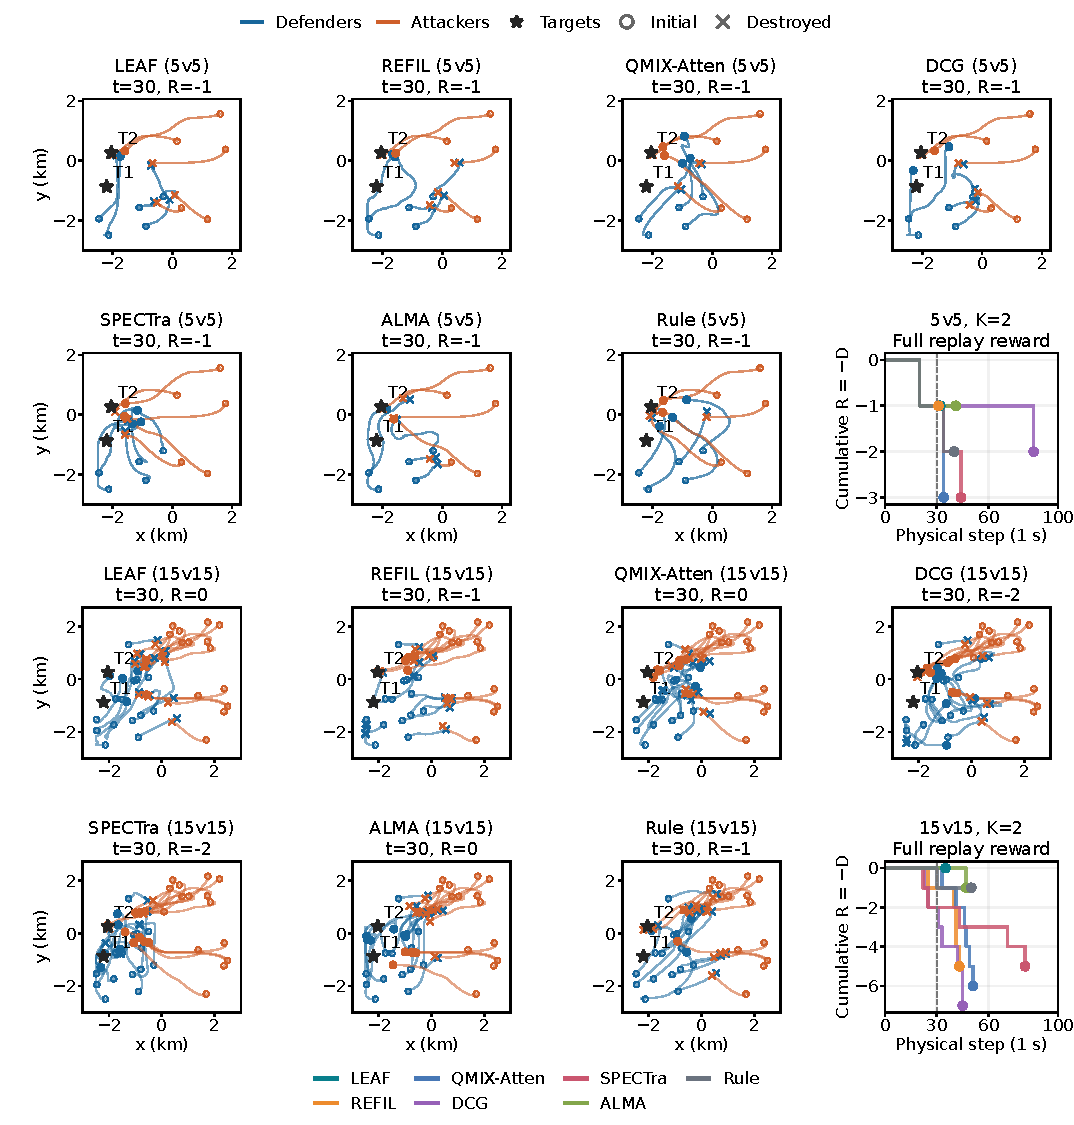
\includegraphics[width=\textwidth]{figures/fig_leaf_final1007_trajectory.pdf}
\caption{Seven-method trajectories on preselected scene 9000: the upper two rows show 5v5 and the lower two rows show 15v15, both with two targets. Each block contains seven spatial panels and a shared cumulative-reward plot. Learned policies use final checkpoints from training seed 0. Paths end at the common snapshot step 30; open circles show initial positions, filled circles show live vehicles, crosses show destroyed vehicles, and stars show targets. Spatial titles give reward at the snapshot. Reward curves continue to each actual terminal step, marked by a dot; the dashed line marks the snapshot. Entity colors and spatial limits are shared within each scale.}
\label{fig:had-cases}
\end{figure*}

\section{Conclusion}
LEAF separates contextual entity processing within a decision from temporal recurrence across decisions. A shared loop develops receiver-relative entity context, learned fusion combines intermediate reads, and a downstream GRU maintains memory. Query-history input is zero and explicit count injection is disabled. Frozen LEAF policies achieve higher group mean reward $R=-D$ than five learning baselines and Rule across the four evaluated HAD population groups. The saved memory-query comparison favors LEAF at the group-mean level while both designs retain downstream recurrence.

On the three-configuration diagnostic subset, reading the initial workspace without contextual updates lowers all nine seed--configuration reward means despite retaining the relation projection and GRU. The first two rounds receive 98.59--98.91\% of average fusion weight, but most two-round action changes occur among low-margin decisions. Fixing empirical fusion weights has mixed reward effects at $K=2$ and lowers all three seed means at $(30,30,12)$; state-dependent weighting has a consistent advantage in that tested target-rich configuration. GRU reset lowers eight of nine means. These results identify conditional reliance of the saved policies on contextual features, read selection, and temporal state, rather than separate gains from retraining each component. Depth effects remain mixed, and the local action-stability condition does not guarantee closed-loop reward. The evidence concerns a fixed simulated deployment family; transfer across adversary strategies and physical operating conditions remains to be established.

\appendices
\section{Complete Design-Variant Context}
The ten completed variants share the formal scene matrix and three training seeds. Table~\ref{tab:had-full-variants} preserves the selection context. Last uses only the final read, Fixed4 uses four rounds in both training and execution, ARR anchors keys and values at the initial workspace, Untied4 uses distinct round blocks, and Looped + count enables typed-count injection. These five variants use historical-query inputs. Their results characterize complete trained designs. Saved optimizer settings match for LEAF and + Memory query; the seed-1 runs used collection concurrency 12 and 6, respectively, so their sampled training histories are not controlled to be identical.
\HadFullVariantTable
\section{Learning-Record Sources}
\label{app:learning-source}
LEAF and the design references use main0928 HAD validation records. An untrimmed main0923 snapshot supplies 105,000 native validation episodes for seven baseline methods, preserving source-version main0921: three training seeds, 50 checkpoints, four configurations, and 25 scenes per configuration. Five baselines enter the main learning plot; REFIL-matched and TransfQMix are additional references. All 21 baseline last-point means and environment-step counts match archived checkpoint progress. Curves use native records, without PDF-derived values or retraining. Configuration imports retain only HAD settings. Supplementary pursuit records with different outcomes are kept separate; the pursuit analysis uses canonical main0928 records.
\section{Local Replay Provenance}
\label{app:replay}
The original auxiliary runs record HAD Workbench 2.1.0; added loop/fusion runs record SkyHAD 3.0.0 and the new trajectories 3.0.0rc2. Their protocol labels differ. The 90 standard recaptures match initial states and 11 outcome fields, supporting the local paired controls rather than establishing full runtime equivalence.
All 90 REFIL and 77 of 90 LEAF standard replays match 11 archived fields: reward, length, termination, per-target damage and first-damage steps, surviving populations, death causes, collisions, and action histograms. The 13 differences concern LEAF seed 2: four scenes at $(10,10,2)$ and nine at $(50,50,2)$, including five reward differences. For the first divergent scene, GPU execution with and without diagnostics gives identical actions and values; CPU execution gives the same actions and outcome. The historical cause remains unresolved because the archived runtime/source snapshot is incomplete. Each intervention therefore uses its local standard control, preserving the formal 300-scene statistics.

The separate seven-method trajectory study uses six registered learned checkpoints and Rule. Eleven of fourteen episodes match all archived fields. At 5v5, DCG has local reward $-2$ and length 86 versus archived $-1$ and 29; ALMA retains reward $-1$ but has length 41 versus 30. At 15v15, ALMA has local reward $-1$ and length 47 versus archived $-2$ and 71. Figure~\ref{fig:had-cases} uses the actual local trajectories and their rewards throughout; no trajectory is combined with an archived outcome from a different rollout.
\section*{Acknowledgment}
OpenAI Codex assisted with manuscript drafting, code-assisted analysis, and figure preparation. The authors are responsible for the methods, numerical results, and final text. All experimental plots in this manuscript use recorded or explicitly identified auxiliary evaluations.
\bibliographystyle{IEEEtran}
\bibliography{references}
\end{document}
